%\documentclass[ignorenonframetext,xcolor=svgnames,hyperref={xetex,colorlinks,linkcolor=blue},compress]{beamer}

\usepackage{pgfpages}

\usepackage{latexsym,pifont,units,amsmath,amsfonts,amssymb,marvosym,wasysym}
\usepackage{xltxtra} %fontspec,xunicode are loaded here.
\defaultfontfeatures{Mapping=tex-text}
\setsansfont{DejaVu Sans}
\setmainfont{DejaVu Serif}

% \usepackage{graphicx} % beamer loads graphicx already.
\graphicspath{{./figs/}{../figs/}{./}{../}} %note that the trailing “/” is required

\usepackage{tikz}
\usetikzlibrary{arrows,decorations.pathmorphing,backgrounds,positioning,fit}

\usepackage{multicol,rotating,soul,varwidth}
\setul{1.5pt}{.4pt}% 1.5pt below contents

\newcommand{\cfbox}[2]{%
  \colorlet{currentcolor}{.}%
  {\color{#1}\fbox{\color{currentcolor}#2}}%
}

\newcommand{\code}[1]{\texttt{\textcolor{violet}{#1}}}

\mode<beamer>{
  \usetheme{default}
  \usecolortheme{sidebartab}
  \usefonttheme{serif}
  % \usefonttheme[onlysmall]{structurebold}
  \setbeamertemplate{footline}[frame number]
  \setbeamertemplate{navigation symbols}{}
  \setbeamertemplate{blocks}[rounded][shadow=true]
  \setbeamercolor{block title}{fg=Green}
  \setbeamercolor{structure}{fg=Green}
}

\begin{document}

\mode<article>{
  \title{Process Scheduling}
  \author{Wang Xiaolin\\wx672ster@gmail.com}
  \maketitle
  \tableofcontents
  \vspace{2em}
  \begin{description}
  \item[Textbooks:] \ \\
    \begin{itemize}
    \item Chapter 4, \emph{Process Scheduling}, \cite{love2010linux}
    \item Chapter 2, \emph{Process Management and Scheduling}, \cite{mauerer2008professional}
    \end{itemize}
  \end{description}
  \printbibliography
  \clearpage
}

\begin{frame}<beamer>
  \title{Process Scheduling}
  \author{Wang Xiaolin}
  \titlepage
  \vfill
  \tiny{
    \ding{41} wx672ster@gmail.com
    % \ding{37} 
  }
\end{frame}

\section{Multitasking}
\label{sec:multitasking}

\begin{frame}{Multitasking}
  \begin{enumerate}
  \item Cooperative multitasking
    \begin{description}
    \item[Yielding] a process voluntarily suspends itself
    \end{description}
  \item Preemptive multitasking
    \begin{description}
    \item[Preemption] involuntarily suspending a running process
    \item[Timeslice] the time a process runs before it's preempted
      \begin{itemize}
      \item usually dynamically calculated
      \item used as a configurable system policy
      \end{itemize}
      But Linux's scheduler is different
    \end{description}
  \end{enumerate}
\end{frame}

\section{Linux's Process Scheduler}
\label{sec:linuxs-proc-sched}

\begin{frame}{Linux's Process Scheduler}
  \begin{description}
  \item[up to 2.4:] simple, scaled poorly
    \begin{multicols}{2}
      \begin{itemize}
      \item $O(n)$
      \item non-preemptive
      \item single run queue (cache? SMP?)
      \end{itemize}
    \end{multicols}
  \item[from 2.5 on:] $O(1)$ scheduler
    \begin{itemize}
    \item 140 priority lists --- scaled well
    \item one run queue per CPU --- true SMP support
    \item preemptive
    \item ideal for large server workloads
    \item showed latency on desktop systems
    \end{itemize}
  \item[from 2.6.23 on:] Completely Fair Scheduler (CFS)
    \begin{itemize}
    \item improved interactive performance
    \end{itemize}
  \end{description}
\end{frame}

\begin{description}
\item[up to 2.4:] (Sec 7.2, \emph{The Scheduling Algorithm},
  \cite{bovet2005understanding}) The scheduling algorithm used in earlier versions of
  Linux was quite simple and straightforward: at every process switch the kernel scanned
  the list of runnable processes, computed their priorities, and selected the "best"
  process to run. The main drawback of that algorithm is that the time spent in choosing
  the best process depends on the number of runnable processes; therefore, the algorithm
  is too costly, that is, it spends too much time in high-end systems running thousands of
  processes.
  \begin{description}
  \item[No true SMP] all processes share the same run-queue
  \item[Cold cache] if a process is re-scheduled to another CPU
  \end{description}
\end{description}

\section{Scheduling Policy}
\label{sec:scheduling-policy}

\begin{frame}{Scheduling Policy}
  Must attempt to satisfy two conflicting goals:
  \begin{enumerate}
  \item fast process response time (low latency)
  \item maximal system utilization (high throughput)
  \end{enumerate}
  \vspace{1em}
  
  Linux tries
  \begin{enumerate}
  \item favoring I/O-bound processes over CPU-bound processes
  \item doesn't neglect CPU-bound processes
  \end{enumerate}
\end{frame}

\begin{frame}{Process Priority}
  Usually,
  \begin{itemize}
  \item processes with a higher priority run before those with a lower priority
  \item processes with the same priority are scheduled \emph{round-robin}
  \item processes with a higher priority receive a longer time-slice
  \end{itemize}
\end{frame}

\begin{frame}
    Linux implements two priority ranges:
  \begin{enumerate}
  \item \textbf{Nice value}: $-20 \sim+19$ (default 0)
    \begin{itemize}
    \item large value $\Rightarrow$ lower priority
    \item lower value $\Rightarrow$ higher priority  $\Rightarrow$ get larger proportion
      of a CPU
    \end{itemize}
    \begin{center}
      $\sim$\$ \code{ps -el}
    \end{center}
    The \emph{nice value} can be used as 
    \begin{itemize}
    \item a control over the \emph{absolute} time-slice (e.g. MAC OS X), or
    \item a control over the \emph{proportion} of time-slice (Linux)
    \end{itemize}
  \item \textbf{Real-time}: $0\sim99$
    \begin{itemize}
    \item higher value $\Rightarrow$ greater priority
    \end{itemize}
    \begin{center}
      \mbox{$\sim$\$ \code{ps -eo state,uid,pid,rtprio,time,comm}}
    \end{center}
  \end{enumerate}
\end{frame}

\begin{frame}{Time-slice}
  \begin{description}
  \item[too long:] poor interactive performance
  \item[too short:] context switch overhead
  \item[I/O-bound processes:] don't need longer time-slices (prefer short queuing time)
  \item[CPU-bound processes:] prefer longer time-slices (to keep their caches hot)
  \end{description}
  Apparently, any long time-slice would result in poor interactive performance.
\end{frame}

\begin{frame}{Problems With Nice Value}
  \begin{multicols}{2}
    \code{if} two processes A and B
    \begin{itemize}
    \item[A:] $NI=0, t=100ms$
    \item[B:] $NI=20, t=5ms$
    \end{itemize}\vfill\columnbreak
    \code{then}, the CPU share
    \begin{itemize}
    \item[A:] gets $\frac{100}{105} = 95\%$
    \item[B:] gets $\frac{5}{105} = 5\%$
    \end{itemize}
  \end{multicols}
  \begin{block}{What if two $B_{ni=20}$ running?}
    \begin{description}
    \item[Good news:] Each gets $50\%$
    \item[Bad news:] This '50\%' is $\frac{5}{10}$, NOT $\frac{52.5}{105}$
    \end{description}
    Context switch twice every 10ms!
  \end{block}
\end{frame}
\clearpage
\begin{frame}
  \begin{multicols}{2}
    Comparing
    \begin{itemize}
    \item[] $P_{ni=0}$ gets 100ms
    \item[] $P_{ni=1}$ gets 95ms
    \end{itemize}\vfill\columnbreak
    With
    \begin{itemize}
    \item[] $P_{ni=19}$ gets 10ms
    \item[] $P_{ni=20}$ gets 5ms
    \end{itemize}
  \end{multicols}
  This behavior means that ``nicing down a process by one'' has wildly different effects
  depending on the starting nice value.
\end{frame}

\subsection{Linux's CFS}
\label{sec:linuxs-cfs}

\begin{frame}{Completely Fair Scheduler (CFS)}
  For a perfect (unreal) multitasking CPU
  \begin{itemize}
  \item $n$ runnable processes can run at the same time
  \item each process should receive $\frac{1}{n}$ of CPU power
  \end{itemize}
  
  For a real world CPU
  \begin{itemize}
  \item can run only a single task at once --- unfair
    \begin{itemize}
    \item[\Smiley] while one task is running
    \item[\Frowny\Frowny] the others have to wait
    \end{itemize}
  \item \code{p->wait\_runtime} is the amount of time the task should now run on the CPU
    for it becomes completely fair and balanced.
    \begin{itemize}
    \item[\Smiley] on ideal CPU, the \code{p->wait\_runtime} value would always be zero
    \end{itemize}
  \item CFS always tries to run the task with the largest \code{p->wait\_runtime} value
  \end{itemize}
\end{frame}

\begin{itemize}
\item \href{http://kerneltrap.org/node/8208}{kerneltrap: Linux: Discussing the Completely
    Fair Scheduler}
\end{itemize}

\begin{frame}{CFS}
  In practice it works like this:
  \begin{itemize}
  \item While a task is using the CPU, its \code{wait\_runtime} decreases
    \begin{center}
      \code{wait\_runtime = wait\_runtime - time\_running}
    \end{center}
  \item[if:] its \code{$\mathtt{wait\_runtime} \ne \mathtt{MIN}_{wait\_runtime}$}
    (among all processes)
  \item[then:] it gets preempted
  \item Newly woken tasks (\code{wait\_runtime = 0}) are put into the tree more and more
    to the right
  \item slowly but surely giving a chance for every task to become the 'leftmost task' and
    thus get on the CPU within a deterministic amount of time
  \end{itemize}
\end{frame}

\begin{frame}
  \begin{center}
    \mode<beamer>{
      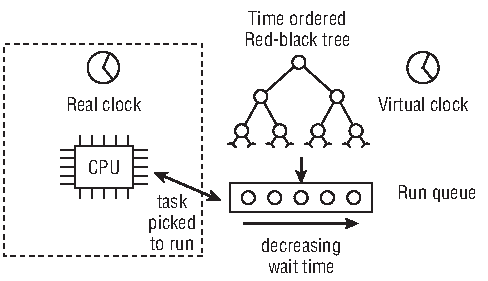
\includegraphics[width=\textwidth]{cfs1}
    } \mode<article>{
      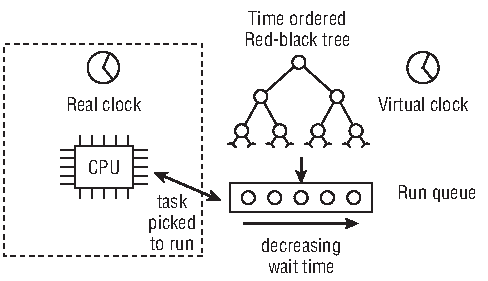
\includegraphics[width=.5\textwidth]{cfs1}
    }
  \end{center}
  \begin{itemize}
  \item the run queue is sorted by waiting time with a red-black tree
  \item the leftmost node in the tree is picked by the scheduler
  \end{itemize}
\end{frame}

\begin{itemize}
\item (p84, \cite{mauerer2008professional}) An outstanding feature of the Linux scheduler
  is that it does not require the concept of time slices, at least not in the traditional
  way. Classical schedulers compute time slices for each process in the system and allow
  them to run until their time slice is used up. When all time slices of all processes
  have been used up, they need to be recalculated again. The current scheduler, in
  contrast, considers only the wait time of a process --- that is, how long it has been
  sitting around in the run-queue and was ready to be executed. The task with the gravest
  need for CPU time is scheduled.

  ... but what do \emph{fair} and \emph{unfair} with respect to CPU time mean? Consider an
  ideal computer that can run an arbitrary number of tasks in parallel: If $N$ processes
  are present on the system, then each one gets $\frac{1}{N}$ of the total computational
  power, and all tasks really execute physically parallel. Suppose that a task requires 10
  minutes to complete its work. If 5 such tasks are simultaneously present on a perfect
  CPU, each will get 20 percent of the computational power, which means that it will be
  running for 50 instead of 10 minutes. However, all 5 tasks will finish their job after
  exactly this time span, and none of them will have ever been inactive!

  If multitasking is simulated by running one process after another, then the process that
  is currently running is favored over those waiting to be picked by the scheduler --- the
  poor waiting processes are being treated unfairly. The unfairness is directly
  proportional to the waiting time.

  Every time the scheduler is called, it picks the task with the highest waiting time and
  gives the CPU to it. If this happens often enough, no large unfairness will accumulate
  for tasks, and the unfairness will be evenly distributed among all tasks in the system.
\end{itemize}


\begin{frame}{The virtual clock}
  Time passes slower on this clock than in real time
  \begin{itemize}
  \item[] more processes waiting $\Rightarrow$ more slower
  \end{itemize}
  \begin{block}{Example}
    \begin{itemize}
    \item[if:] 4 processes in run queue
    \item[then:] the virtual clock speed is $\frac{1}{4}$ of the real clock
    \item[if:] a process sitting in the queue for 20s in real time
    \item[then:] resulting to 5s in virtual time
    \item[if:] the 4 processes executing for 5s each
    \item[then:] the CPU will be busy for 20s in real time
    \end{itemize}
  \end{block}
\end{frame}

\begin{itemize}
\item The virtual clock is a per process clock. Whenever the CPU comes, this
  clock starts ticking. And it stops ticking immediately when the CPU is going away.
\end{itemize}

\begin{frame}
  \begin{block}{To sort tasks on the red-black tree}
    \begin{center}
      \cfbox{violet}{\code{fair\_clock - wait\_runtime}}
    \end{center}
    \begin{description}
    \item[\code{fair\_clock}] The virtual time, e.g. 5s in the previous example
    \item[\code{wait\_runtime}] Fairness imbalance measure 
    \end{description}
  \end{block}
  \begin{block}{To move a node rightward in the red-black tree}
    \begin{center}
      \cfbox{violet}{\code{wait\_runtime = wait\_runtime - time\_running}}
    \end{center}
    \begin{description}
    \item[\code{time\_running}] When a task is allowed to run, the interval during which
      it has been running
    \end{description}
  \end{block}
\end{frame}

\begin{frame}{CFS}
  \begin{block}{Example: }
    Assuming \emph{targeted latency} is 20ms. If we have
    \begin{description}
    \item[2 processes:] each gets 10ms
    \item[4 processes:] each gets 5ms
    \item[20 processes:] each gets 1ms
    \item[$\infty$ processes:] each gets 1ms (to avoid unacceptable context switching costs)
    \end{description}
  \end{block}
\end{frame}

\begin{itemize}
\item Sec \emph{The Linux Scheduling Algorithm}, p49, \cite{love2010linux}
\end{itemize}

% \begin{frame}{Linux's CFS}
%   \begin{itemize}
% %  \item Doesn't require the concept of time-slices
%   \item Assign a \emph{proportion} of CPU to processes
%     \begin{itemize}
%     \item[] rather than directly assign time-slices to processes
%     \end{itemize}
%   \item The amount of CPU time that a process receives is a function of the load of the
%     system
%   \item The nice value acts as a \emph{weight}
%   \end{itemize}
  
%   \begin{itemize}
%   \item[Q:] Can a runnable process immediately preempt the running process?
%   \item[A:] CFS decides it based on \emph{the percentage of CPU the newly runnable process
%     has consumed}.
%     \begin{itemize}
%     \item[if:] it has consumed a smaller proportion than the running process
%     \item[then:] it runs immediately
%     \item[else:] it is scheduled to run at a later time
%     \end{itemize}
%   \end{itemize}
% \end{frame}

\begin{frame}{Example}
  A system with two processes running:
  \begin{enumerate}
  \item a text editor, say, Emacs (I/O-bound)
  \item gcc is compiling the kernel source (CPU-bound)
  \end{enumerate}
  \begin{itemize}
  \item[if:] they both have the same nice value
  \item[then:] the proportion they get would be 50\%-50\%
  \end{itemize}
  Consequence:
  \begin{itemize}
  \item Emacs uses far less than 50\% of CPU
  \item gcc can enjoy more than 50\% of CPU freely
  \end{itemize}
  When Emacs wakes up
  \begin{enumerate}
  \item CFS notes that it has 50\% of CPU, but uses very little of it (far less than gcc)
  \item CFS preempts gcc and enables Emacs to run immediately
  \end{enumerate}
  Thus, better interactive performance.
\end{frame}

\section{Linux Scheduling Algorithm}
\label{sec:linux-sched-algor}

\begin{frame}{Scheduler Classes}
  Different, pluggable algorithms coexist 
  \begin{itemize}
  \item Each algorithm schedules its own type of processes
  \item Each scheduler class has a priority
  \end{itemize}
  \begin{description}
  \item[\code{SCHED\_FIFO}]
  \item[\code{SCHED\_RR}]
  \item[\code{SCHED\_NORMAL}] 
  \end{description}
\end{frame}

\begin{frame}
  \begin{block}{Example: nice value difference}
    Assume:
    \begin{enumerate}
    \item nice value 5 pts up results in a $\frac{1}{3}$ penalty
    \item targeted latency is again 20ms
    \item 2 processes in the system
    \end{enumerate}
    Then:
    \begin{itemize}
    \item $P_{ni=0}$ gets 15ms; $P_{ni=5}$ gets 5ms
    \item $P_{ni=10}$ gets 15ms; $P_{ni=15}$ gets 5ms
    \end{itemize}
    \begin{itemize}
    \item Absolute nice values no longer affect scheduling decision
    \item Relative nice values does
    \end{itemize}
  \end{block}
\end{frame}

\begin{itemize}
\item p49, \cite{love2010linux}
\end{itemize}

\section{The Linux Scheduling Implementation}
\label{sec:linux-sched-impl}

Sec 4.5, \emph{The Linux Scheduling Implementation}, \cite{love2010linux}

\begin{itemize}
\item \href{https://en.wikipedia.org/wiki/Completely_Fair_Scheduler}{Wikipedia: Completely
  Fair Scheduler}
\item \href{http://www.ibm.com/developerworks/linux/library/l-cfs/}{IBM developerworks:
    Multiprocessing with the Completely Fair Scheduler}
\item
  \href{http://embeddeddev.wordpress.com/2011/11/23/scheduling-in-the-linux-kernel/}{Scheduling
    in the Linux kernel – RSDL/SD}
\item \href{http://kerneltrap.org/node/8059}{kerneltrap: Linux: The Completely Fair
    Scheduler}
\end{itemize}

\begin{itemize}
\item Sec 7.2, \cite{bovet2005understanding}.
\end{itemize}

\begin{frame}{Base Time Quantum}
  \begin{block}{$O(1)$ scheduler}
    \begin{scriptsize}
      \begin{equation*}
        \genfrac{}{}{0pt}{}{\text{base time quantum}}{(\text{ms})}=
        \begin{cases}
          (140 - \text{static priority})\times{}20& if\ \text{static priority} < 120,\\
          (140 - \text{static priority})\times{}5& if\ \text{static priority} \ge 120.
        \end{cases}
      \end{equation*}
    \end{scriptsize}
  \end{block}
\end{frame}

\begin{frame}{Major Components of CFS}
  \begin{itemize}
  \item Time Accounting
  \item Process Selection
  \item The Scheduler Entry Point
  \item Sleeping and Waking Up
  \end{itemize}
\end{frame}


\begin{frame}{Time accounting}
  \begin{description}
  \item[\code{sched\_entity}] keeps track of process accounting (\code{task\_struct -> se})
  \end{description}
  \begin{center}
    \mode<beamer>{
      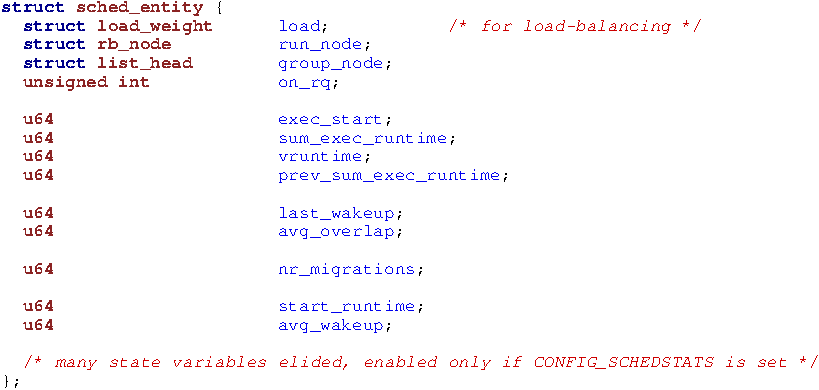
\includegraphics[width=\textwidth]{se}
    } \mode<article>{
      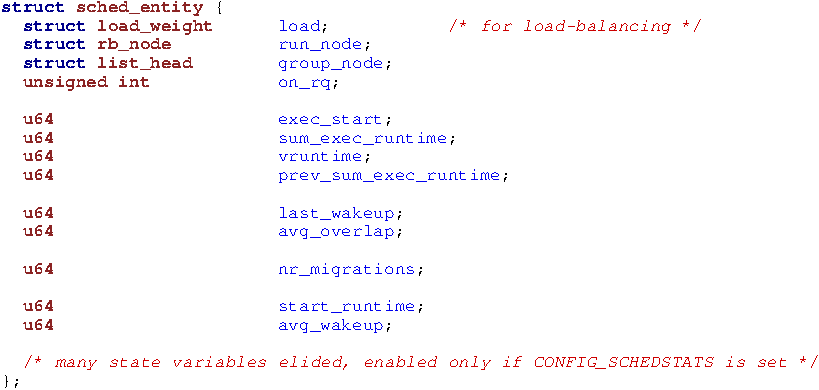
\includegraphics[width=.7\textwidth]{se}
    }
  \end{center}
\end{frame}

\begin{frame}
  \begin{block}{The Virtual Runtime}
    \begin{description}
    \item[\code{vruntime}] stores the \emph{virtual runtime} of a process. On an ideal
      processor, all tasks' \code{vruntime} would be identical.
    \end{description}
    Accounting is done in \code{update\_curr()} and \code{\_\_update\_curr()}
  \end{block}
\end{frame}

\begin{itemize}
\item \code{update\_curr()} (line
  \href{http://lxr.linux.no/linux+v2.6.34/kernel/sched_fair.c#L518}{518} in
  \code{kernel/sched\_fair.c}) 
\item \code{\_\_update\_curr()} (line
  \href{http://lxr.linux.no/linux+v2.6.34/kernel/sched_fair.c#L503}{503} in
  \code{kernel/sched\_fair.c}) 
\item p51-p52, \cite{love2010linux}
\end{itemize}

\begin{frame}{Process Selection}
  \begin{description}
  \item[The core of CFS algorithm] Pick the process with the smallest \code{vruntime}
  \end{description}
  \begin{itemize}
  \item run the process represented by the leftmost node in the \code{rbtree}
  \end{itemize}
  \begin{center}
    \mode<beamer>{
      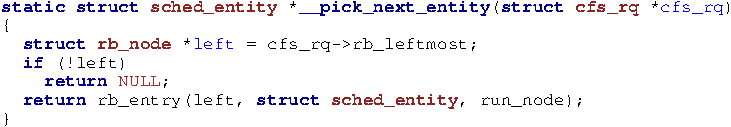
\includegraphics[width=\textwidth]{pick-next-entity}
    } \mode<article>{
      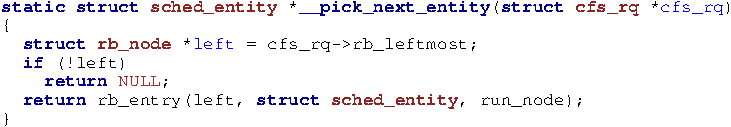
\includegraphics[width=.8\textwidth]{pick-next-entity}
    }
  \end{center}
\end{frame}

\begin{frame}{Adding Processes to the Tree}
  \begin{itemize}
  \item Happens when a process wakes up or is created
  \item \code{enqueue\_entity()} and \code{\_\_enqueue\_entity()}
  \end{itemize}
\end{frame}

\begin{itemize}
\item p54-55, \cite{love2010linux}
\end{itemize}

\begin{frame}{Removing Processes from the Tree}
  \begin{itemize}
  \item Happens when a process blocks or terminates
  \item \code{dequeue\_entity()} and \code{\_\_dequeue\_entity()}
  \end{itemize}
\end{frame}

\begin{frame}{The Scheduler Entry Point}
  
\end{frame}

\begin{frame}{Sleeping and Waking Up}
  
\end{frame}

\end{document}
% (setq-default TeX-master nil)
